%%% Preamble
\documentclass{report}

\usepackage[utf8]{inputenc}
\usepackage[T1]{fontenc}
\usepackage{fourier}
\usepackage[french]{babel}
\usepackage[protrusion=true,expansion=true]{microtype}	
\usepackage{amsmath,amsfonts,amsthm} % Math packages
\usepackage[pdftex]{graphicx}	
\usepackage{url}
\usepackage{pdfpages}
\usepackage{todonotes}
\usepackage[a4paper, body={16cm,26cm}]{geometry}
\usepackage{float}
\usepackage{framed}
\usepackage[toc,page]{appendix} 
\usepackage{multicol}
\usepackage{colortbl}
\usepackage{epstopdf}
\usepackage{adjustbox}

%%% Custom sectioning
\usepackage{sectsty}
\allsectionsfont{  \normalfont\scshape}
%\allsectionsfont{\centering \normalfont\scshape}

%%% Custom headers/footers (fancyhdr package)
\usepackage{fancyhdr}
\pagestyle{fancyplain}
\fancyhead{}								% No page header
\fancyfoot[L]{}							% Empty 
\fancyfoot[C]{}							% Empty
\fancyfoot[R]{\thepage}					% Pagenumbering
\renewcommand{\headrulewidth}{0pt}		% Remove header underlines
\renewcommand{\footrulewidth}{0pt}		% Remove footer underlines
\setlength{\headheight}{13.6pt}


%%% Equation and float numbering
\numberwithin{equation}{section}		% Equationnumbering: section.eq#
\numberwithin{figure}{section}		% Figurenumbering: section.fig#
\numberwithin{table}{section}		% Tablenumbering: section.tab#


%%% Define new commands
\newcommand{\horrule}[1]{\rule{\linewidth}{#1}} 	% Horizontal rule
\renewcommand{\bf}[1]{\textbf{#1}}
\renewcommand{\it}[1]{\textit{#1}}
\newcommand{\bfit}[1]{\textbf{\textit{#1}}}
\renewcommand{\sc}[1]{\textsc{#1}}

\newcommand{\Todo}[1]{\todo[inline]{#1}}
\renewcommand{\thesection}{\thepart .\arabic{section}}

\usepackage{tocloft}
\cftsetindents{chapter}{0em}{1em}
\cftsetindents{section}{1.5em}{2.5em}
\makeatletter
\def\l@figure{\@dottedtocline{1}{1.5em}{4em}}
\makeatother

\usepackage{bookmark}
%\usepackage[hidelinks]{hyperref}
\usepackage{cases}
\usepackage{color}
\usepackage{xcolor}
\usepackage{relsize}
\usepackage{caption}
\colorlet{shadecolor}{black!10}

\delimitershortfall-1sp
\newcommand\abs[1]{\left|#1\right|}


\usepackage{tikz, pgfplots}


%}}}
%{{{ --- pgfplots ---------------------

%{{{ Colors

% TolColors from http://www.r-bloggers.com/the-paul-tol-21-color-salute/
\definecolor{TolColor1}{HTML}{332288}   % dark purple
\definecolor{TolColor2}{HTML}{6699CC}   % dark blue
\definecolor{TolColor3}{HTML}{88CCEE}   % light blue
\definecolor{TolColor4}{HTML}{44AA99}   % light green
\definecolor{TolColor5}{HTML}{117733}   % dark green
\definecolor{TolColor6}{HTML}{999933}   % dark brown
\definecolor{TolColor7}{HTML}{DDCC77}   % light brown
\definecolor{TolColor8}{HTML}{661100}   % dark red
\definecolor{TolColor9}{HTML}{CC6677}   % light red
\definecolor{TolColor10}{HTML}{AA4466}  % light pink
\definecolor{TolColor11}{HTML}{882255}  % dark pink
\definecolor{TolColor12}{HTML}{AA4499}  % light purple

%}}}
%{{{ Color cycles

\pgfplotscreateplotcyclelist{mbarplot cycle}{%
  {draw=TolColor2, fill=TolColor2!70},
  {draw=TolColor7, fill=TolColor7!70},
  {draw=TolColor4, fill=TolColor4!70},
  {draw=TolColor11, fill=TolColor11!70},
  {draw=TolColor1, fill=TolColor1!70},
  {draw=TolColor8, fill=TolColor8!70},
  {draw=TolColor6, fill=TolColor6!70},
  {draw=TolColor9, fill=TolColor9!70},
  {draw=TolColor10, fill=TolColor10!70},
  {draw=TolColor12, fill=TolColor12!70},
  {draw=TolColor3, fill=TolColor3!70},
  {draw=TolColor5, fill=TolColor5!70},
}

\pgfplotscreateplotcyclelist{mlineplot cycle}{%
  {TolColor2, mark=*, mark size=1.5pt},
  {TolColor7, mark=square*, mark size=1.3pt},
  {TolColor4, mark=triangle*, mark size=1.5pt},
  {TolColor6, mark=diamond*, mark size=1.5pt},
}


\pgfplotsset{
  compat=1.9,
  mbaseplot/.style={
    legend style={
      draw=none,
      fill=none,
      cells={anchor=west},
    },
    x tick label style={
      font=\footnotesize
    },
    y tick label style={
      font=\footnotesize
    },
    legend style={
      font=\footnotesize
    },
    major grid style={
      dotted,
    },
    axis x line*=bottom,
  },
  mlineplot/.style={
    mbaseplot,
    xmajorgrids=true,
    ymajorgrids=true,
    major grid style={dotted},
    axis x line=bottom,
    axis y line=left,
    legend style={
      cells={anchor=west},
      draw=none
    },
    cycle list name=mlineplot cycle,
  },
  mbarplot base/.style={
    mbaseplot,
    bar width=6pt,
    axis y line*=none,
  },
  mbarplot/.style={
    mbarplot base,
    ybar,
    xmajorgrids=false,
    ymajorgrids=true,
    area legend,
    legend image code/.code={%
      \draw[#1] (0cm,-0.1cm) rectangle (0.15cm,0.1cm);
    },
    cycle list name=mbarplot cycle,
  },
  horizontal mbarplot/.style={
    mbarplot base,
    xmajorgrids=true,
    ymajorgrids=false,
    xbar stacked,
    area legend,
    legend image code/.code={%
      \draw[#1] (0cm,-0.1cm) rectangle (0.15cm,0.1cm);
    },
    cycle list name=mbarplot cycle,
  },
  disable thousands separator/.style={
    /pgf/number format/.cd,
      1000 sep={}
  },
}


%%  ========   IMPORTANT ========
%% Spécifier ici les variables pour le document
\newcommand{\mainTitle}{\'Etude préalable - SPIE}
\newcommand{\secondTitle}{\'Etude de l'\'Existant}
\newcommand{\documentRef}{DEB-EE/4401/1}
\newcommand{\auteurs}{
Lisa \textsc{Courant} \\
Estelle \textsc{Lepeigneux} \\
Pierre \textsc{Jarsaillon} \\
Hugues \textsc{Verlin} \\
}
\newcommand{\chefDeProjet}{Paul \textsc{Dautry}}
\newcommand{\responsableQualite}{Antoine \textsc{Chabert}}

%%% Begin document
\begin{document}
%----------------------------------------------------------------------------------------
%	PACKAGES
%----------------------------------------------------------------------------------------

\documentclass[12pt]{article}
\usepackage[a4paper]{geometry}
\geometry{verbose,tmargin=1in,bmargin=0in,lmargin=1in,rmargin=1in}
\usepackage[utf8]{inputenc}
\usepackage[francais]{babel}
\usepackage[T1]{fontenc}

\usepackage{graphicx}
\begin{document}

\begin{titlepage}

\newcommand{\HRule}{\rule{\linewidth}{0.5mm}} % horizontal lines

\center % Center everything
 
%----------------------------------------------------------------------------------------
%	HEADING SECTIONS
%----------------------------------------------------------------------------------------

\vspace*{1cm}

\textsc{\LARGE INSA de LYON}\\[1.5cm] 
\textsc{\Large D\'epartement Informatique}\\[0.5cm] 
\textsc{\large Projet Longue Durée}\\[0.5cm] % 

%----------------------------------------------------------------------------------------
%	TITLE SECTION
%----------------------------------------------------------------------------------------

\HRule \\[0.4cm]
{ \huge \bfseries Compte Rendu}\\[0.1cm]
{\large \bfseries - Gestion des contacts commerciaux d'une banque -} 
\HRule \\[1.5cm]
 
%----------------------------------------------------------------------------------------
%	DATE SECTION
%----------------------------------------------------------------------------------------

{\large \today}\\[2cm] % 
 
%----------------------------------------------------------------------------------------
%	AUTHOR SECTION
%----------------------------------------------------------------------------------------

\begin{minipage}{0.4\textwidth}
\begin{center} \large
\emph{Auteurs} \\
Lisa \textsc{Courant} \\
Estelle \textsc{Lepeigneux} \\
Pierre \textsc{Jarsaillon} \\
Hugues \textsc{Verlin} \\
\end{center}
\end{minipage}
~
\begin{minipage}{0.4\textwidth}
\begin{center} \large
\emph{Chef de projet} \\
Paul \textsc{Dautry}
\end{center}
\begin{center} \large
\emph{Responsable Qualité} \\
Antoine \textsc{Chabert}
\end{center}
\end{minipage}\\[5cm]

H4401\\[2cm]

%----------------------------------------------------------------------------------------
%	LOGO SECTION
%----------------------------------------------------------------------------------------

\includegraphics[scale=0.3]{figures/logo.png}
%----------------------------------------------------------------------------------------

\vfill % Fill the rest of the page with whitespace

\end{titlepage}
\end{document}


%% Commenter les deux lignes suivantes pour le document final
%\listoftodos
%\newpage

%% Table de matière / figures / tableaux
\tableofcontents
\listoffigures
\listoftables
\newpage

%%
\part{Contexte}
\setcounter{section}{0}
Cette étude, réalisée pour la société SPIE Sud-Est s'inscrit dans un projet de plus grande ampleur. Elle ne constitue en effet que la première étape d'un long processus de refonte des processus et du système d'information de l'entreprise SPIE Sud-Est. \\

Cette étude consistera en l'analyse des processus existant de SPIE ainsi que l'étude des solutions concurrentes afin d'élaborer deux solutions pour refondre le système d'information de SPIE Sud-Est et par la même occasion éventuellement modifier ces processus internes de fonctionnement. \\

Ce document constitue l'étape de synthèse des éléments existant dans l'organisation SPIE Sud-Est, il a pour but de faire un bilan sur le système d'information et les processus tels qu'ils existent au moment où cette étude à lieu. Il décrit également l'ensemble des solutions techniques et informatiques déjà mises en place dans la société pour répondre aux attentes de cette dernière. \\

Ce document doit aussi permettre d'évaluer l'état de la société SPIE et d'identifier des axes d'amélioration. Il sera complété par la suite par deux documents qui sont décrit dans la suite.

Le premier document constitue l'évaluation des solutions mises en place par les concurrents de SPIE si ces informations sont accessibles. Il présentera également les différents progiciels disponibles sur le marché et s'appuiera sur des processus formalisés afin d'évaluer l'adéquation de ces derniers avec les attentes de SPIE.

Le deuxième réalisera la synthèse des deux premiers en décrivant les pistes d'amélioration dégagées de l'étude de l'existant et du benchmarking précédemment réalisés. Il proposera alors une spécification de la cible à atteindre lors de la phase suivante qui consiste en l'élaboration de deux solutions. 
%%
\part{Périmètre fonctionnel}
\setcounter{section}{0}

Notre étude se limite, en terme de périmètre fonctionnel, à l'activité de Maintenance de la société SPIE Sud-Est. Les deux sections suivantes apportent des précisions sur cette société.

\section{Présentation générale de SPIE Sud-Est}

SPIE Sud-Est est une filiale régionale de services multitechniques de SPIE Opérations sur le quart sud-est de la France.

\begin{figure}[H]
    \label{fig-implem-spie}
    \noindent\makebox[\textwidth]{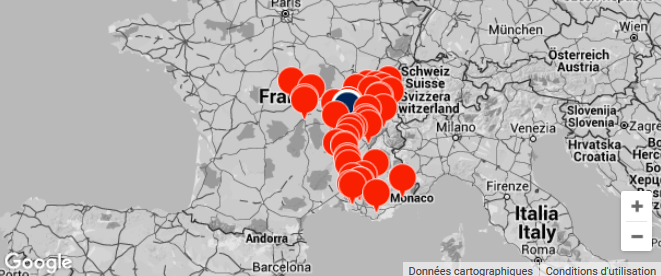
\includegraphics[width=10cm]{figures/implentations_spie.png}}
    \caption{Cartographie des implémentations de SPIE Sud-Est}
\end{figure}

Elle propose à ses clients un service de proximité et une offre diversifiée dans les domaines de l'énergie et des communications et les accompagne dans la conception, la réalisation, l’exploitation et la maintenance d’installations économes en énergie et respectueuses de l’environnement

\section{Organisation géographique et métiers de SPIE Sud-Est}

Du point de vue de l'organisation géographique, la société SPIE Sud-Est est organisée en territoires qui sont parmis les suivants : \\
\begin{itemize}
    \item[\textbullet] Rhône Alpes Auvergne
    \item[\textbullet] Espace Lémanique
    \item[\textbullet] Grand Dauphiné
    \item[\textbullet] Provence Alpes Côte d'Azur\\
\end{itemize}
    
La société SPIE Sud-Est remplit des missions dans les secteurs suivants :  \\
\begin{itemize}
    \item[\textbullet] Maintenance tertiaire
    \item[\textbullet] Génie climatique
    \item[\textbullet] Services aux industries
    \item[\textbullet] Télécoms services
    \item[\textbullet] Infrastructure / énergie \& transport
\end{itemize}
%%
\part{Description du système d'information organisé}
\setcounter{section}{0}
\section{Présentation des processus métiers}

\begin{description}
\item \bf{Offre et revue d'offre} : Un appel d'offre est lancé, donc une opportunité de contrat de service est saisie. Après analyse, ils peuvent faire suite ou non à cet appel d'offre. \\

\item \bf{Négociation client} : Ce processus n'est pour l'instant pas décrit, on le verra dans un second temps avec les axes d'amélioration. \\

\item \bf{Commande et revue de commande} : Si l'offre a été validée avec le client, il faut réaliser la revue du dossier de commande et négocier avec le client. \\

\item \bf{Lancement des prestations de service et travaux} : On lance la commande après qu'elle ait été accepté. Il faut mobiliser les ressources nécessaires et créer des documents opérationnels pour aboutir à une situation initiale connue. \\

\item \bf{Réalisation de prestations de maintenance} : Il faut exécuter les prestations mises en place. Une revue périodique de contrat est effectuée pour ensuite se diriger vers les évolutions du contrat. \\

\item \bf{Réalisation travaux induits} : On réalise tous les travaux éventuellement induits par ce qui a été effectué précédemment. S'il n'y en a pas, on passe à la suite. \\

\item \bf{\'Evolution du contrat} : Le contrat peut éventuellement évoluer après analyse des risques. \\

\item \bf{Solde de l'affaire et du contrat} : Une fois que tout a été effectué, on va clore le contrat et archiver tous les documents.
\end{description}

\section{Détail des différents processus}

\subsection{Offre et revue d'offre}

À la suite d'un appel d'offres, une opportunité de contrat de service est saisie. Il faut également réaliser une opportunité d'avenant, faisant sortir l'entreprise du cadre de maintenance corrective pour aller vers un cadre de maintenance évolutive. Le directeur opérationnel et le responsable d'activité maintenance décideront de la saisie de l'opportunité, tandis que le directeur opérationnel et le commercial donneront leur avis. S'ils décident de ne pas la saisir, le pilote de l'offre indiquera au client qu'ils ne souhaitent pas poursuivre. À l'inverse, si l'opportunité est saisie, il faut tout d'abord collecter des données (à la responsabilité du pilote de l'offre), puis les analyser avec l'aide éventuelle de la direction des ressources humaines et du service juridique (entres autres). \\

Après analyse, le pilote de l'offre peut décider de décliner la proposition et de confirmer au client que l'opportunité ne sera pas saisie. Dans le cas contraire, une réponse positive sera donnée au client. Il faut alors créer et enregistrer le dossier auprès du secrétariat de maintenance, puis proposer des solutions avec le calcul du prix de revient. Enfin, il faudra choisir la solution la plus adaptée ainsi et les prix de vente retenus. Il faut ensuite rédiger l'offre initiale et la faire valider en interne, pour finalement la transmettre dans les délais impartis.


\subsection{Commande et revue de commande}

Après avoir effectué la revue de l'offre, les négociations avec le client sont effectuées. Une fois l'offre validée avec le client, le secrétariat de maintenance l'enregistre et diffuse un original et des copies du dossier de commande. Le responsable d'activité maintenance affecte ensuite la commande au porteur opérationnel en désignant un responsable. Une fois la revue de commande effectuée, le responsable d'affaire valide les données nouvelles après avoir réalisé un plan d'action de validation. Il faut ensuite négocier avec le client, et les deux parties pourront soit trouver un accord et accepter la commande, soit la refuser s'ils n'arrivent pas à trouver un terrain d'entente. Quelle que soit l'issue de la négociation, le service commercial référence le contrat et son état.

\subsection{Lancement des prestations de service et travaux}

Si la commande a été acceptée, il faut la lancer. Les spécifications client sont connues, et on dispose de toutes les données internes nécessaires, le responsable d'affaire peut alors prendre en compte le dossier contractuel et le dossier d'étude. Le RA va alors analyser les exigences et les besoins, et identifier les acteurs afin de faire valider l'organigramme. \\

Une réunion de lancement a alors lieu, réunion pour laquelle seront présents tous les acteurs majeurs du contrat : RA, responsable opérationnel contrat (ROC), service des méthodes, mais aussi éventuellement les commerciaux, le service de gestion, ou encore la direction des ressources humaines, parmi d'autres. Une fois la réunion effectuée, il faut mobiliser les ressources nécessaires pour les rendre disponibles et opérationnelles, avec l'aide indispensable du ROC. En ayant à disposition le dossier de synthèse et les spécifications client, le ROC va créer des procédures et documents opérationnels. Le service des méthodes va alors initialiser des systèmes de gestion. Le responsable d'affaires reprend ensuite la main pour faire le bilan sur tous les actions et documents réalisés jusqu'à présent. Enfin, il va prendre en charge la situation afin d'aboutir à une situation initiale connue et maîtrisée.

\subsection{Réalisation de prestations de maintenance}

La commande de prestations de services et travaux est bien en place : il faut maintenant les exécuter, conformément à la commande et aux documents amonts, sous la responsabilité du responsable activité maintenance. \\

Mais il est également important de gérer l'affaire. Si on dispose de la commande initiale et que tous les documents amonts sont à la disposition du responsable d'affaires, alors la gestion de l'affaire débute dans l'objectif d'obtenir la maîtrise économique et juridique du contrat et de prévoir à nouveau la fin d'affaire. Le RA doit ensuite identifier les avenants (cf. revue d'offre) et les travaux induits (cf. sous-processus "réalisation travaux induits"). \\

Enfin, il faut gérer les activités et le reporting. En ayant à sa disposition les données issues des différents SI, on peut suivre les activités et le reporting client, puis effectuer une revue périodique de contrat grâce à cela, pour se diriger vers les évolutions du contrat.

\subsection{Réalisation travaux induits}

À la suite d'une demande faite par le client ou un intervenant du contrat, on souhaite réaliser des prestations de maintenance et identifier les travaux induits. En étudiant le cahier des charges, le responsable d'affaire va, avec l'aval du responsable opérationnel contrat, décider de donner suite ou non. S'ils décident de ne pas donner suite, il faut en informer le client. \\

Sinon, ils vont ensuite décréter si les travaux sous tous induits. Si ce n'est pas le cas, ces derniers seront redirigés vers le processus Travaux pour que tout soit prêt. Sinon, le RA et le ROC vont se demander si le contrat inclut les modalités d'exécution des travaux induits. Deux cas se présentent alors : \\
\begin{description}
\item Le contrat n'inclut pas les modalités d'exécution. Les travaux sont alors réalisés sur devis. Le RA et le ROC, avec l'aide éventuelle d'autres entités de la société, vont alors directement chiffrer, valider et envoyer ledit devis signé en fonction des pouvoirs. Une fois la commande reçue, elle est validée. \\

\item Le contrat inclut bien des modalités d'exécution. Les travaux sont alors réalisés en dépenses contrôlées, ou bien sur devis (suivant les clauses contractuelles). Le chiffrage et la validation des charges travaux sont ensuite effectués, puis le client est informé, ou on lui envoie un devis. Après réception de la commande orale ou de l'ordre de service, le RA va valider ceci et l'enregistrer sur Supra. \\
\end{description}

La préparation des travaux débute sous la responsabilité du responsable opérationnel contrat. Les consignes d'exécution sont remises au responsable de l'exécution avec les informations sur les éventuels risques et les mesures à prendre. L'exécution des prestations est effectuée, aboutissant à la mise à jour des documents d'exécution. Le client signe alors les documents reçus (PV de réception, CRI\dots), ce qui entraîne le déclenchement de la facture auprès du service Marché, ainsi que la gestion de la garantie.

\subsection{Évolution du contrat}

Grâce à la disponibilité du tableau de bord affaire et activités, des données comptables du système Supra et des différentes orientations (interne et client), le contrat peut évoluer sous la responsabilité du responsable d'affaire. Les risques sont analysés et un bilan de l'affaire est effectué. La décision est ensuite prise de renouveller l'affaire sous sa forme initiale ou sous une autre forme.

\subsection{Solde de l'affaire et du contrat}

L'affaire touche à sa fin : grâce à son bilan, la revue de contrat, les commandes et les avenants, il faut en effectuer la revue. Le client a pu constater des écarts par rapport à ce qui était prévu. Le RA va alors décider de solder les prestations et travaux et d'en effectuer une recette. \\

Un état des lieux de sortie est éventuellement réalisé sous la responsabilité du responsable opérationnel contrat. À la suite de cette réalisation, des écarts peuvent éventuellement être constatés, menant à un plan d'action. Il faut donc traiter ces écarts, et les solder en levant les réserves. \\

Grâce à la recette des prestations travaux et contrat, le responsable d'affaire peut gérer la garantie et en fermer le compte, déterminant la fin de la période de garantie. L'affaire peut alors être soldée et archivée.

\section{Description des données}

\todo{Ajouter le tableau récapitulatif des données mise en jeu dans les processus}

\section{Structure organisationnelle}

\todo{Ajouter un organigramme ARIS}


%%
\part{Description du système informatique}
\setcounter{section}{0}
\section{Applications utilisées par SPIE Sud-Est}

\begin{figure}[H]
    \label{fig-applis-spie}
    \noindent\makebox[\textwidth]{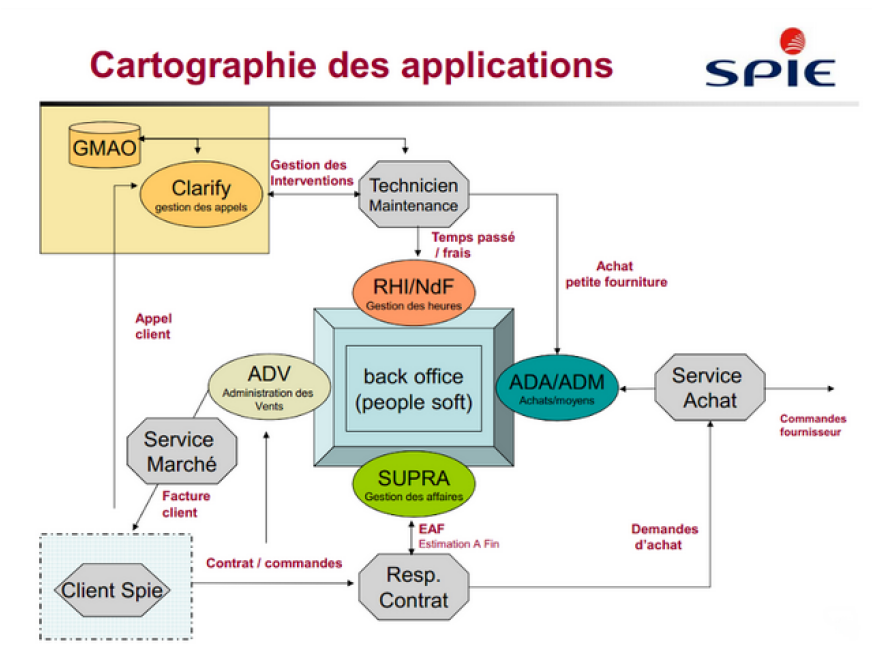
\includegraphics[width=10cm]{figures/applications_spie.png}}
    \caption{Cartographie applicative de SPIE Sud-Est}
\end{figure}

\subsection{People Soft}
Dévéloppé par Oracle et configuré pour répondre à certains des besoins métiers de SPIE.
\begin{description}
    \item \bf{Finalité :} Gestion centralisé de certains processus métiers. \\
    \item \bf{Fonctions :}
    \begin{itemize}
        \item Système de gestion de resources humaines
        \item Financial Mangagement Solution
        \item Customer Relationship Management
        \item Entreprise Performance Management \\
    \end{itemize}
    \item \bf{Utilisateurs :} Tous les utilisateurs des fonctions ci-dessus. \\
    \item \bf{Contraintes :} Ne couvre pas tous les besoins métiers de SPIE et oblige SPIE à avoir d’autres applications spécifique.
\end{description}

\subsection{ADV}
Développement spécifique pour les besoins de SPIE.
\begin{description}
    \item \bf{Finalité :} Administration des ventes. \\
    \item \bf{Fonctions :}
    \begin{itemize}
        \item Enregistrement des commandes de vente
        \item Gestion de la facturation
    \end{itemize}
\end{description}

\subsection{ADA-ADM}
Développement spécifique pour les besoins de SPIE.
\begin{description}
    \item \bf{Finalité :} Administration des achats / Administration des moyens. \\
    \item \bf{Fonctions :}
    \begin{itemize}
        \item Gestion des achats
        \item Gestion des moyens (véhicules / outillages) \\
    \end{itemize}
    \item \bf{Utilisateurs :} Employés du service achat et du service moyens
\end{description}

\subsection{RHI - NDF}
Développement Spécifique pour les besoins de SPIE.
\begin{description}
    \item \bf{Finalité :} Gestion des heures de paies des employés de SPIE. \\
    \item \bf{Fonctions :}
    \begin{itemize}
        \item Sui du pointage des emplyés
        \item Suivi de l’activité hebdomadaires des techniciens de maintenances (tâches effectées, délai et temps d’intervention)
        \item Gestion des notes de frais (saisis des frais liés aux intervention de maintenance, c’est à dire les déplacements ou bien les déjeuners) \\
    \end{itemize}
    \item \bf{Utilisateurs :} Techniciens de maintenance et service comptable. \\
\end{description}

\bf{Observations :} Il faudra fournir un logiciel de meilleur qualité permettant de s’affranchir de Excel.


\subsection{SUPRA}
Développement spécifique pour les besoins de SPIE.
\begin{description}
    \item \bf{Finalité :} Suivi et Gestion pour le responsable d’affaires. \\
    \item \bf{Fonctions :}
    \begin{itemize}
        \item Accès à l’ensemble des informations relatives aux projets du Restponsable d’affaires
        \item Commandes
        \item Dépenses engagées
        \item Factures de fournisseurs
        \item Données internes à l’équipe (heures dépensées par les équipes et coûts associés) \\
    \end{itemize}
    \item \bf{Utilisateurs :} Responsable d’affaires. \\
\end{description}

\bf{Observations :} Certaines fonctions sont aussi présentes dans d’autres outils, il faudrait essayer de faire un peu de “ménage” pour garder que ce qui n’est pas répliqué ailleurs.


\subsection{Clarify}
Développement spécifique pour les besoins de SPIE.
\begin{description}
    \item \bf{Finalité :} Gestion des appels et des demandes d’interventions. \\
    \item \bf{Fonctions :} 
    \begin{itemize}
        \item Gestion (classifications/commentaires) et enregistrement des appels
        \item Traitement des demandes d’intervention et envoi éventuel d’une équipe de maintenance \\
    \end{itemize}
    \item \bf{Utilisateurs :} Agent centre d’appels, responsale de maintenance, techniciens de maintenance
\end{description}

\subsection{Conclusion}

Globalement, l’architecture applicative de la gestion de la maintenance souffre d’une segmentation importance ainsi que de trop nombreux flux. Il peut être nécessaire d’essayer de diminuer la taille de l’architecture applicative en essayant des alternatives qui pourraient couvrir l’ensemble des besoins de SPIE.

\section{Architecture technique de SPIE Sud-Est}

SPIE ne nous a pas fourni d’informations quant à l’organisation de leur architecture technique actuelle. SPIE étant une entreprise de grande taille, nous pouvons supposer que celle-ci supportera les modifications à apporter au SI, étant donné la robustesse de leur SI déjà en place.
Nous savons simplement que la société est orientée autour d’un serveur central auquel chaque filiale française du groupe se connecte.

\section{Bilan des dysfonctionnements de l’existant applicatif et identification des attentes d’amélioration}

\subsection{RHI/NdF}

\noindent\textsc{Dysfonctionnements} : \\

Cette application a pour but de gérer les heures hebdomadaires des techniciens, cependant cette dernière n’est utilisée que par le service gérant les rémunérations des employés. Selon certains responsables, cette application fait preuve de peu de souplesse. Ce manque de souplesse est comblé par des marcos Excel qu’ils utilisent. \\

\noindent\textsc{Attentes d’amélioration} : \\

Il faudrait avoir un outil de qualité intégrant les fonctionnalités que remplissent actuellement les macros qu’ils utilisent sur Excel.

\subsection{SUPRA}


\noindent\textsc{Dysfonctionnements} : \\

SUPRA est un application très ancienne héritant de l’ancien ERP de SPIE. Elle a donc subie de nombreuses modifications et développements spécifiques et présente des dysfonctionnements liés à ces évolutions répétées. \\

\noindent\textsc{Attentes d’amélioration} : \\

Certaines fonctions sont aussi présentes dans d’autres outils, il faudrait essayer de faire un point sur les données gérées par l’application pour éviter la réplication de ces données avec d’autres applications.

\subsection{SI Global}

\noindent\textsc{Dysfonctionnements} : \\

L’architecture actuelle de SPIE est constituée d’un ensemble d’applications qui communiquent les unes avec les autres. Cette disposition entraîne une multiplication des flux et les interdépendances entre les applications ne favorisent pas l’évolutivité du système d’information. \\

\noindent\textsc{Attentes d’amélioration} : \\

Le système d’information de SPIE gagnerait à être plus modulaire, car cela le doterait d’une meilleure évolutivité. Peut être qu’un travail d’intégration de ces fonctionnalités dans une architecture d’entreprise urbanisée permettrait d’atteindre ces objectifs.

%% ANNEXES ---------------------------------------------------------------------------

\appendix
\chapter{Modèle ARIS de l'existant}

\begin{figure}[H]
    \label{fig-gestion-contrats}
    \noindent\makebox[\textwidth]{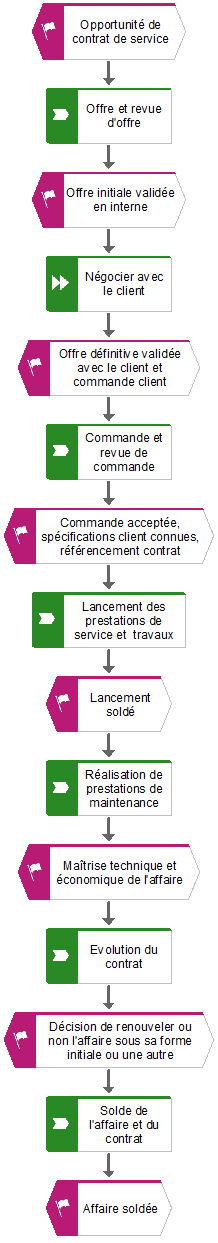
\includegraphics[width=3cm]{figures/aris/gestion_des_contrats_de_maintenances_et_services.png}}
    \caption{Processus Gestion des Contrats de Maintenance et Services}
\end{figure}

\begin{figure}[H]
    \label{fig-offre-revue-offre}
    \noindent\makebox[\textwidth]{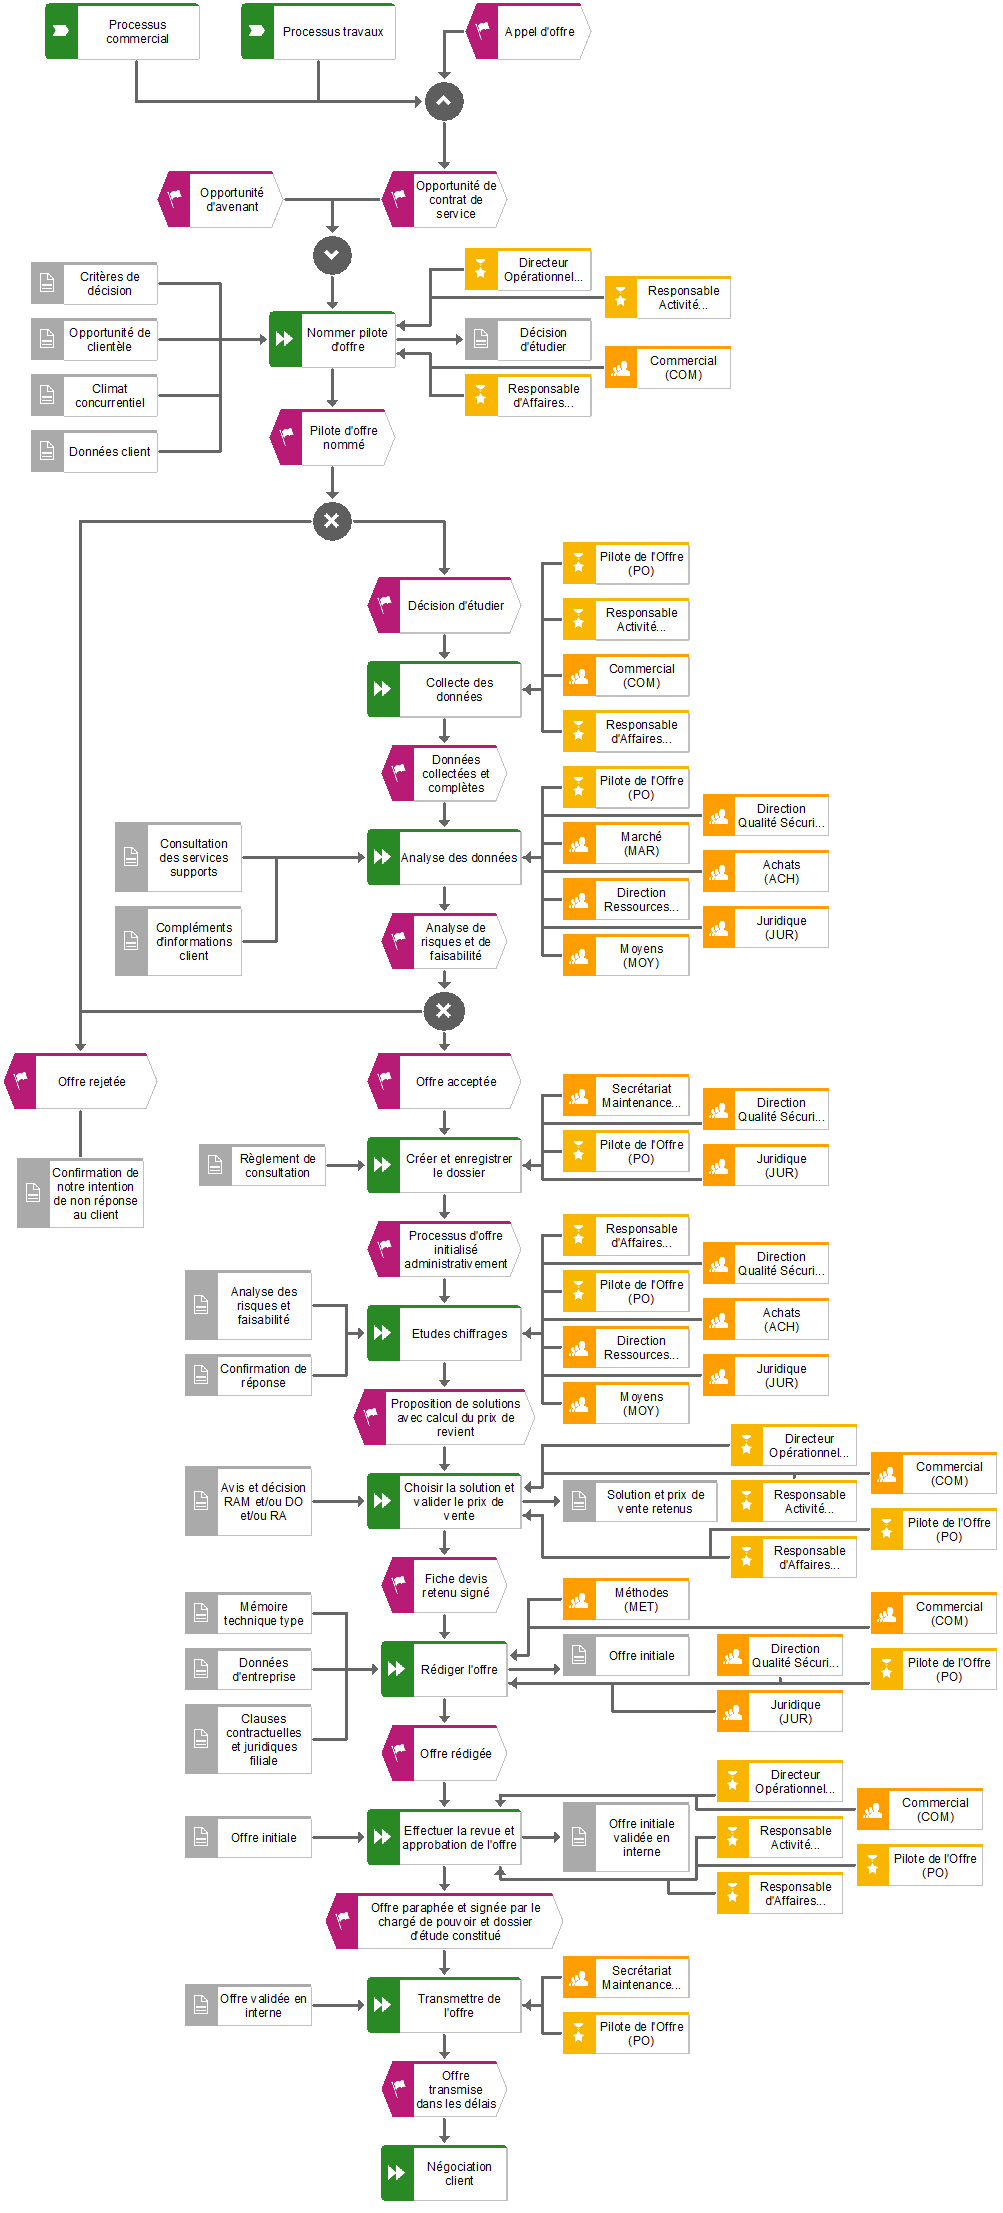
\includegraphics[width=12cm]{figures/aris/offre_et_revue_doffre.png}}
    \caption{Processus Offre et Revue d'Offre}
\end{figure}

\begin{figure}[H]
    \label{fig-commande-revue-commande}
    \noindent\makebox[\textwidth]{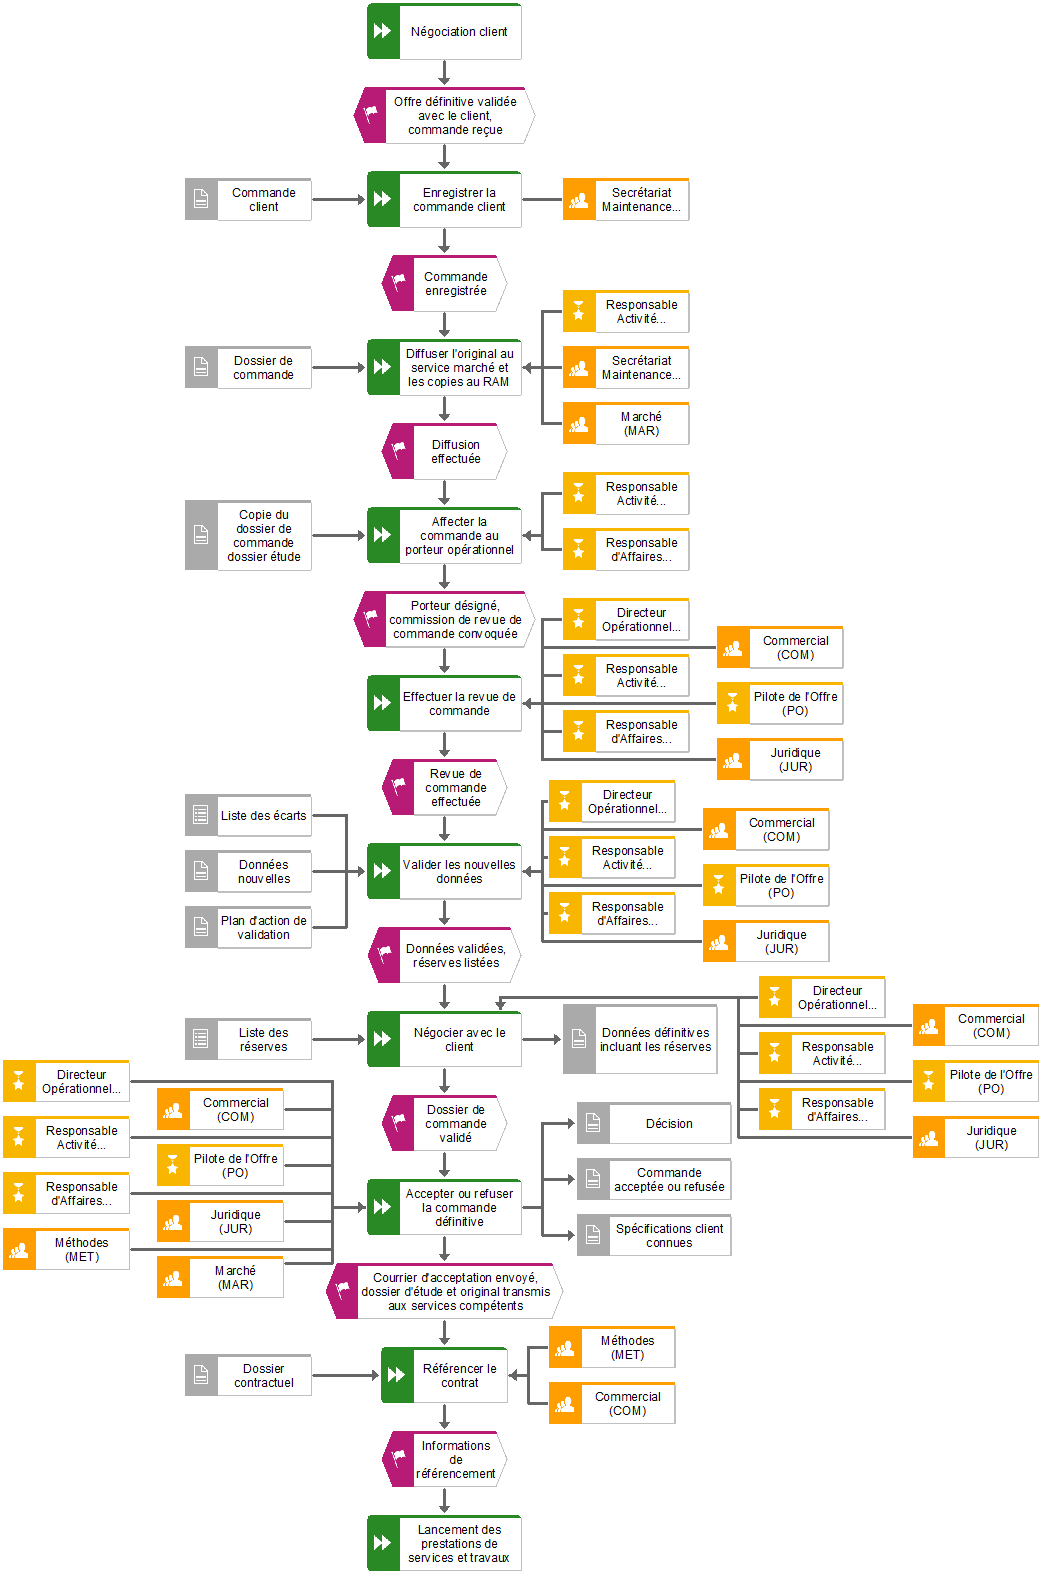
\includegraphics[width=14cm]{figures/aris/commande_et_revue_de_commande.png}}
    \caption{Processus Commande et Revue de Commande}
\end{figure}

\begin{figure}[H]
    \label{fig-lancement-prest}
    \noindent\makebox[\textwidth]{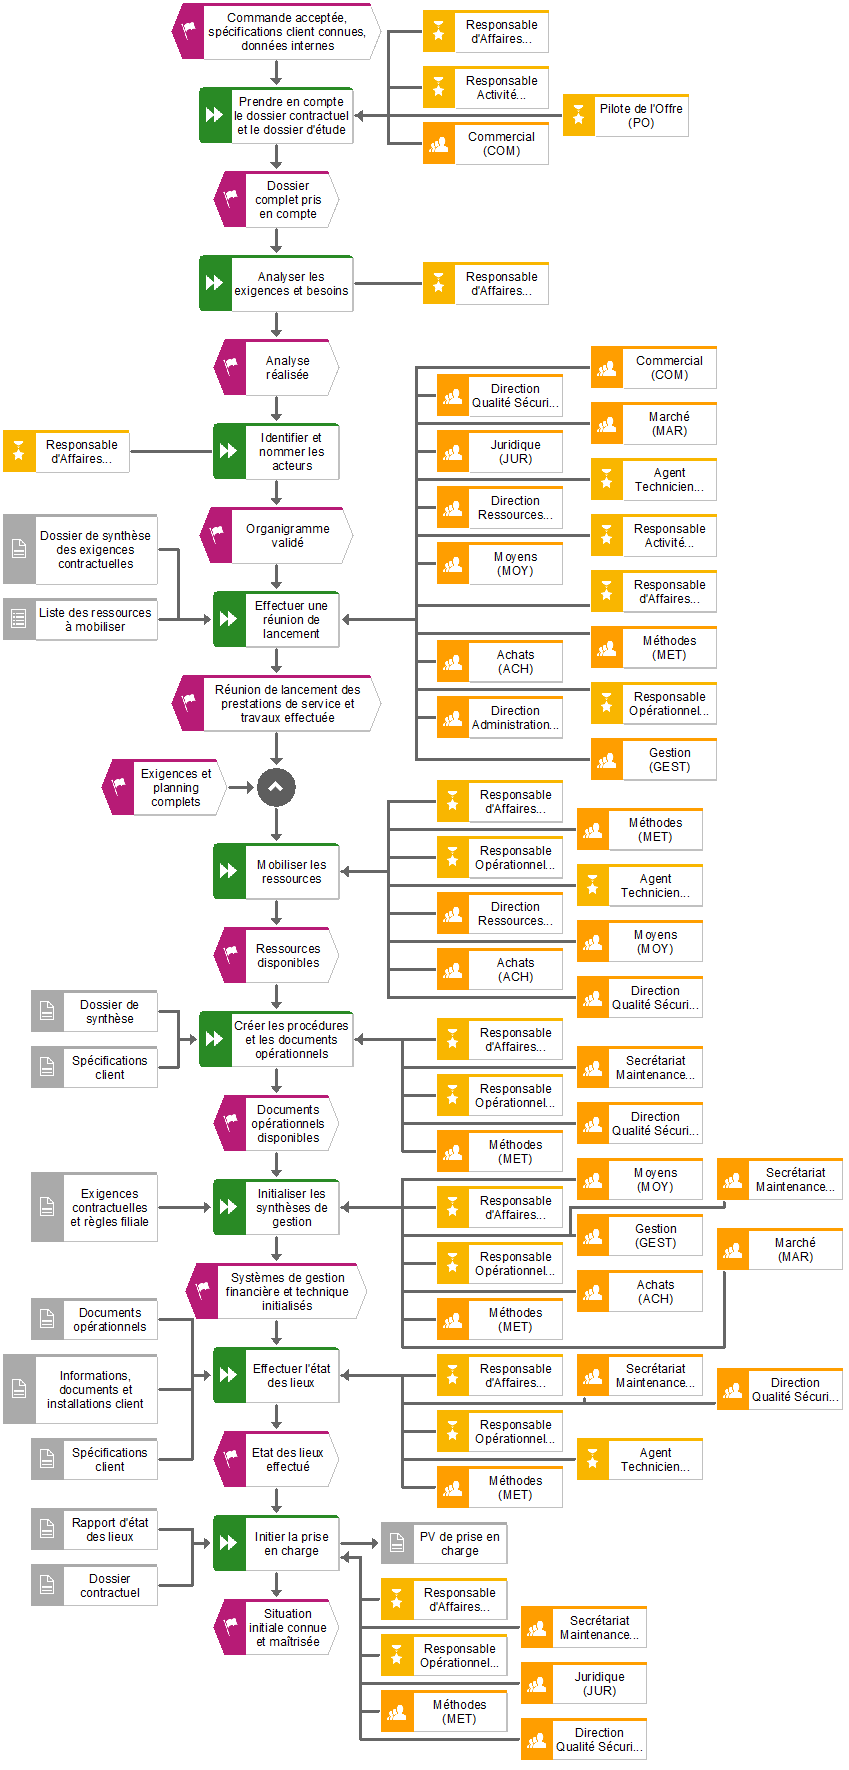
\includegraphics[width=12cm]{figures/aris/lancement_des_prestations_de_services_et_travaux.png}}
    \caption{Processus Lancement des Prestations de Services et Travaux}
\end{figure}

\begin{figure}[H]
    \label{fig-realisation-prest}
    \noindent\makebox[\textwidth]{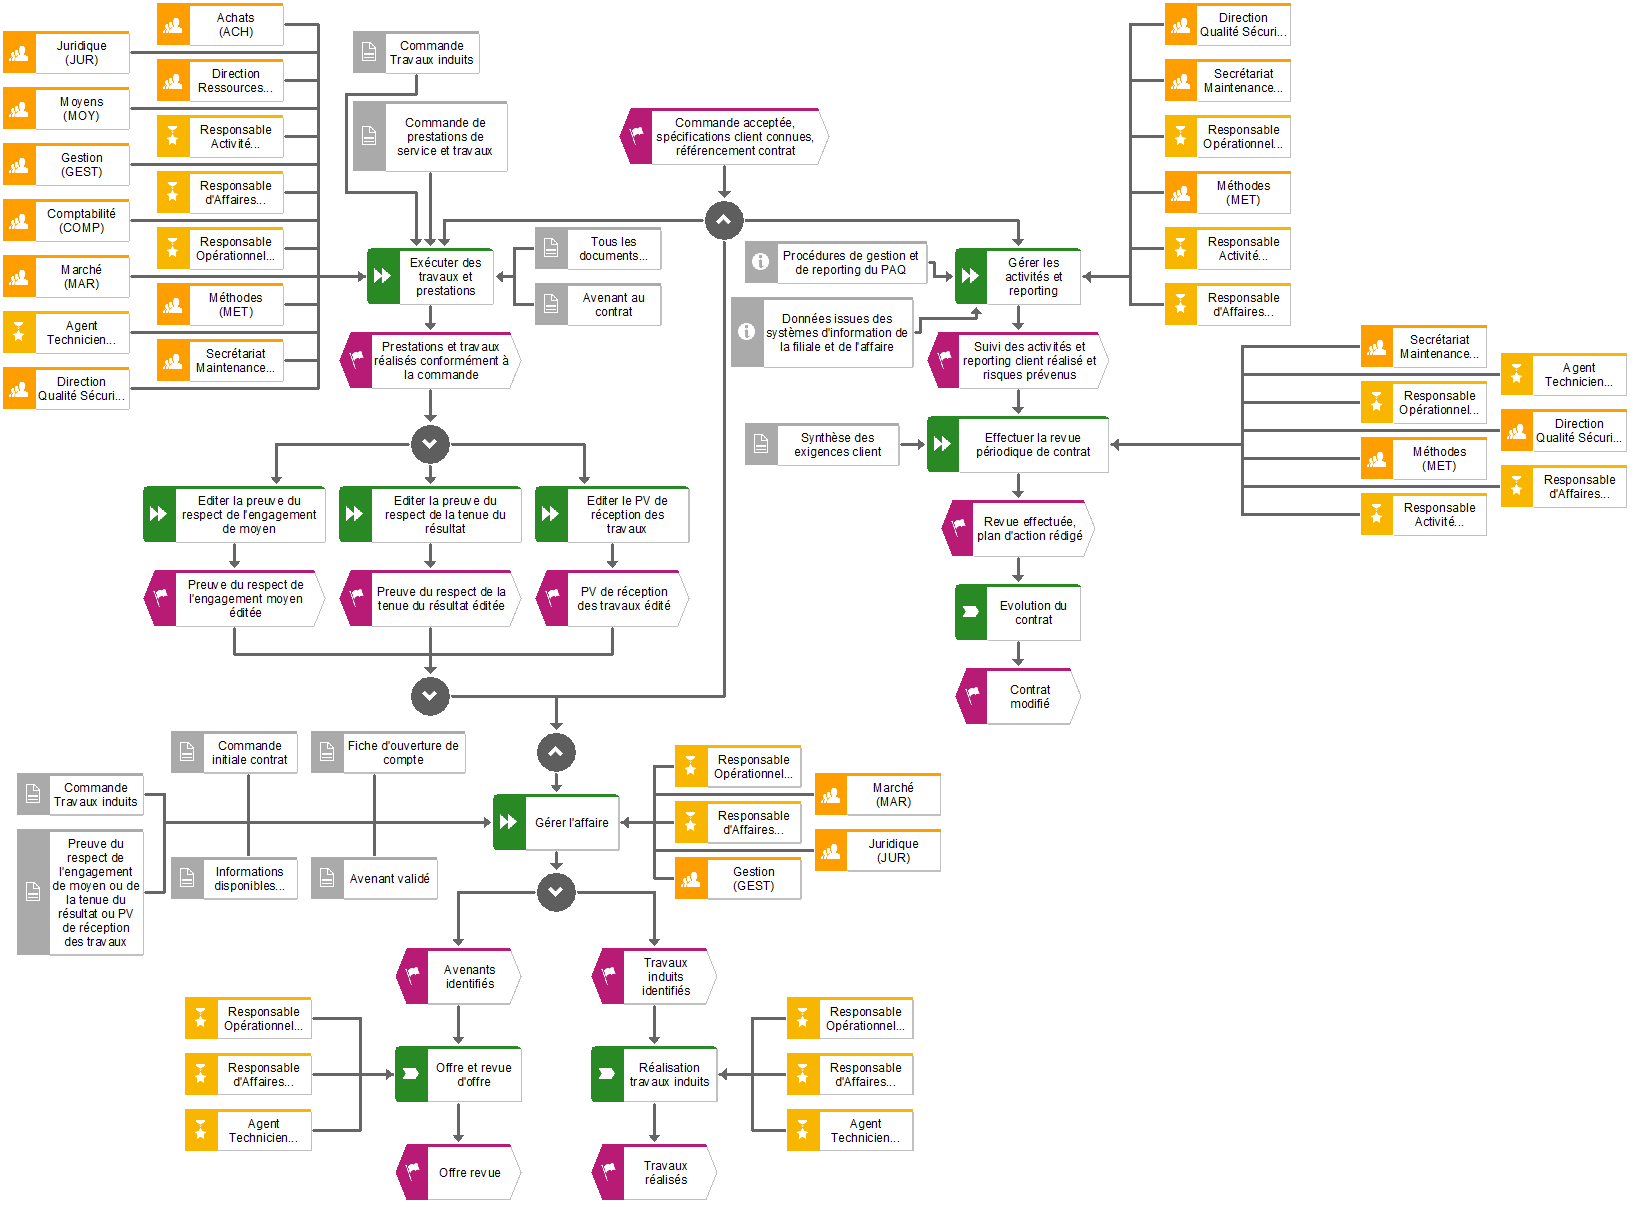
\includegraphics[width=14cm]{figures/aris/realisation_prestations_de_maintenance.png}}
    \caption{Processus Réalisation Prestations de Maintenance}
\end{figure}

\begin{figure}[H]
    \label{fig-travaux-induits}
    \noindent\makebox[\textwidth]{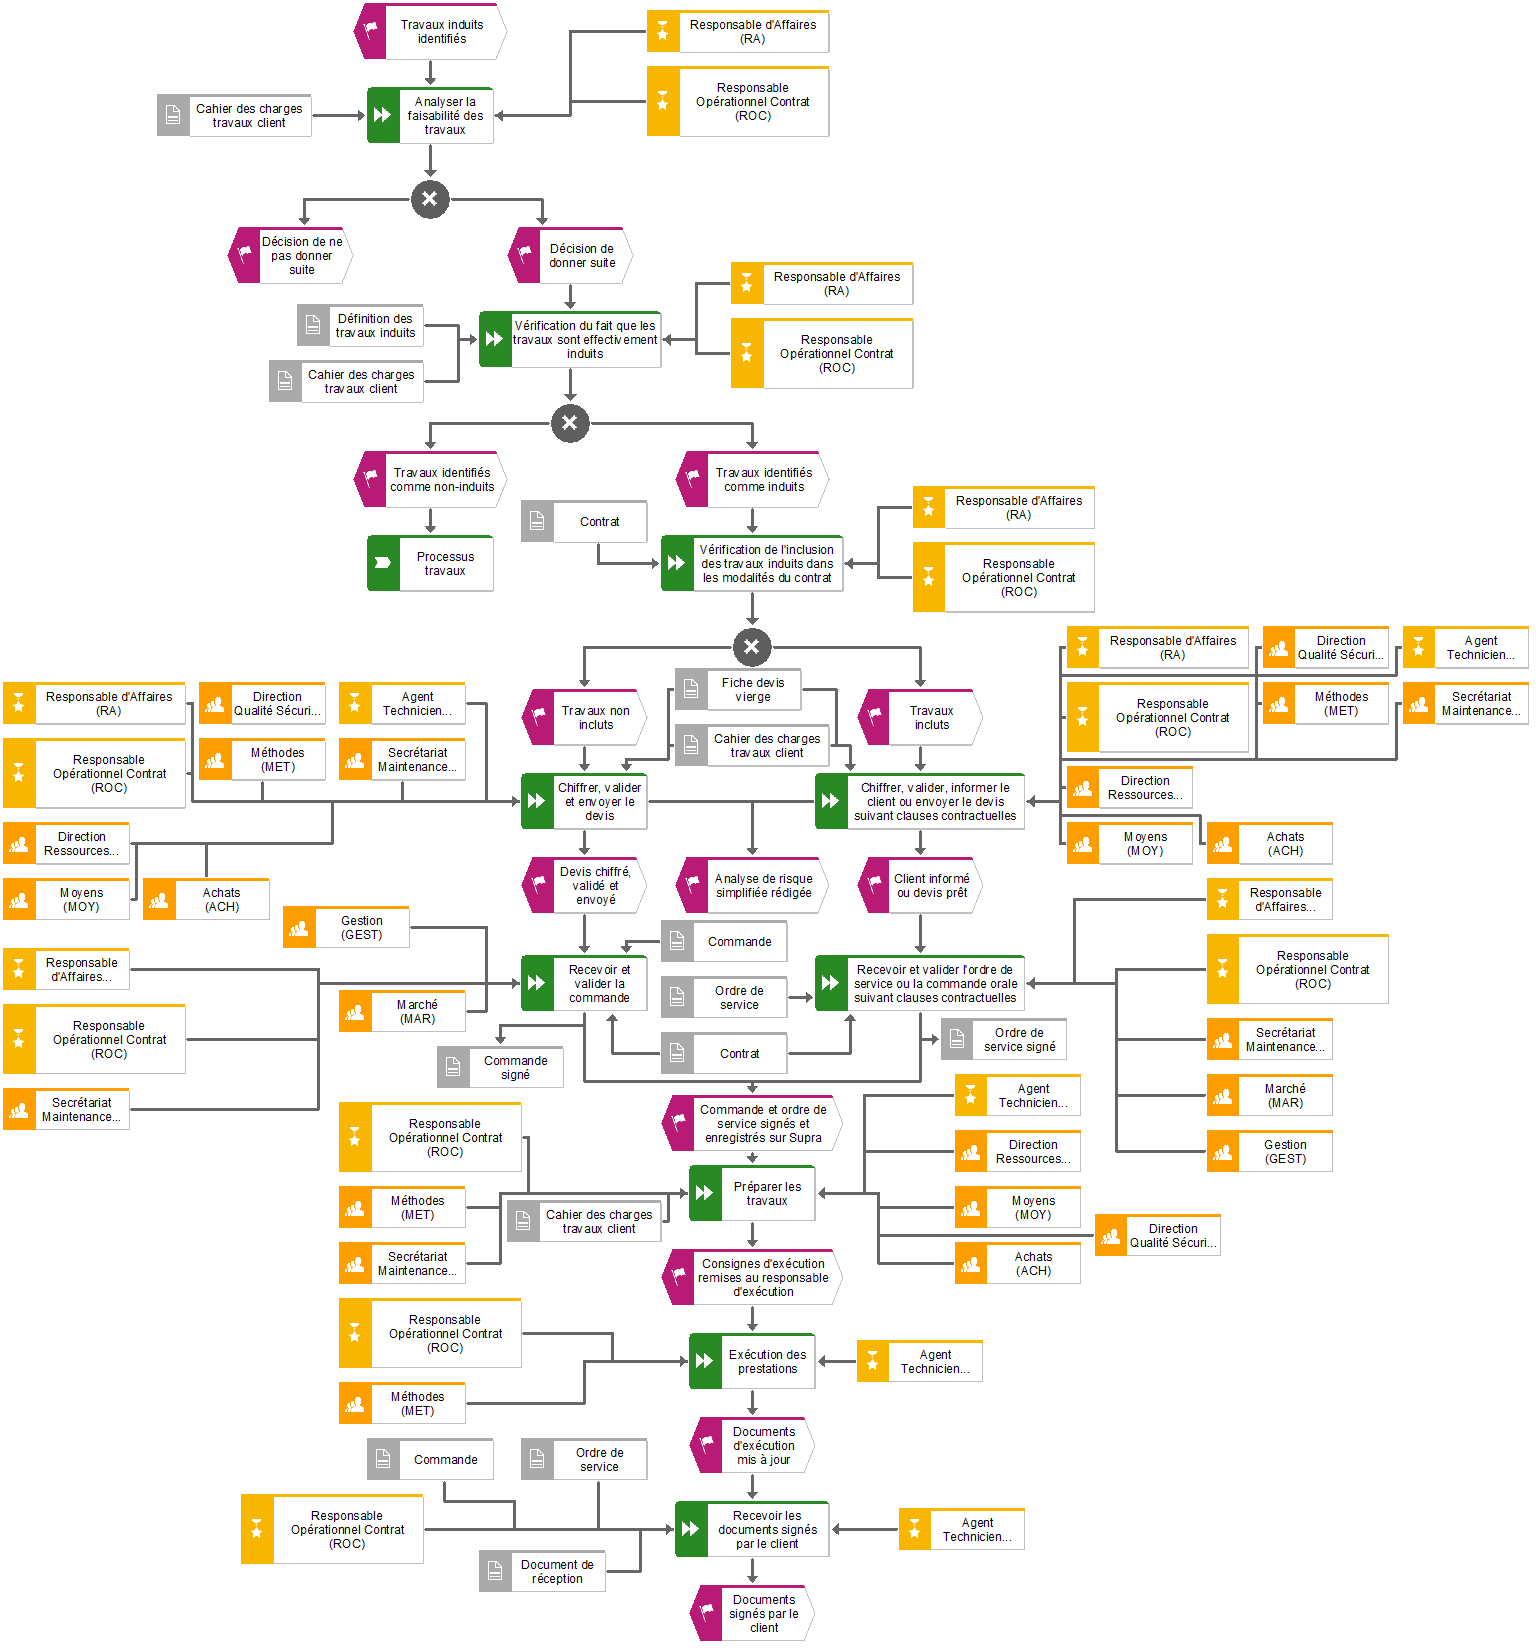
\includegraphics[width=14cm]{figures/aris/realisation_travaux_induits.png}}
    \caption{Processus Réalisation des Travaux Induits}
\end{figure}

\begin{figure}[H]
    \label{fig-evolution-contrat}
    \noindent\makebox[\textwidth]{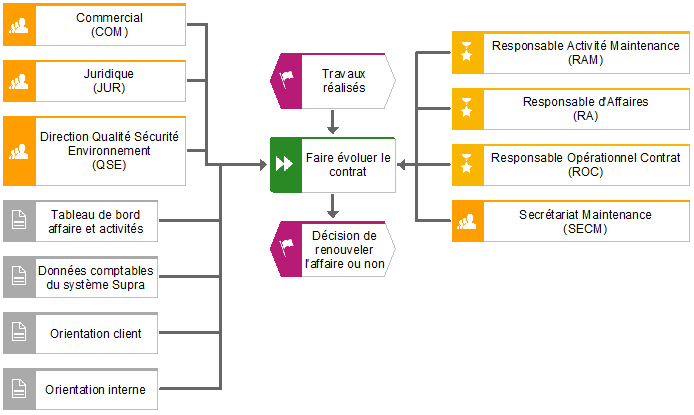
\includegraphics[width=12cm]{figures/aris/evolution_du_contrat.png}}
    \caption{Processus Evolution du Contrat}
\end{figure}

\begin{figure}[H]
    \label{fig-soldes-affaire}
    \noindent\makebox[\textwidth]{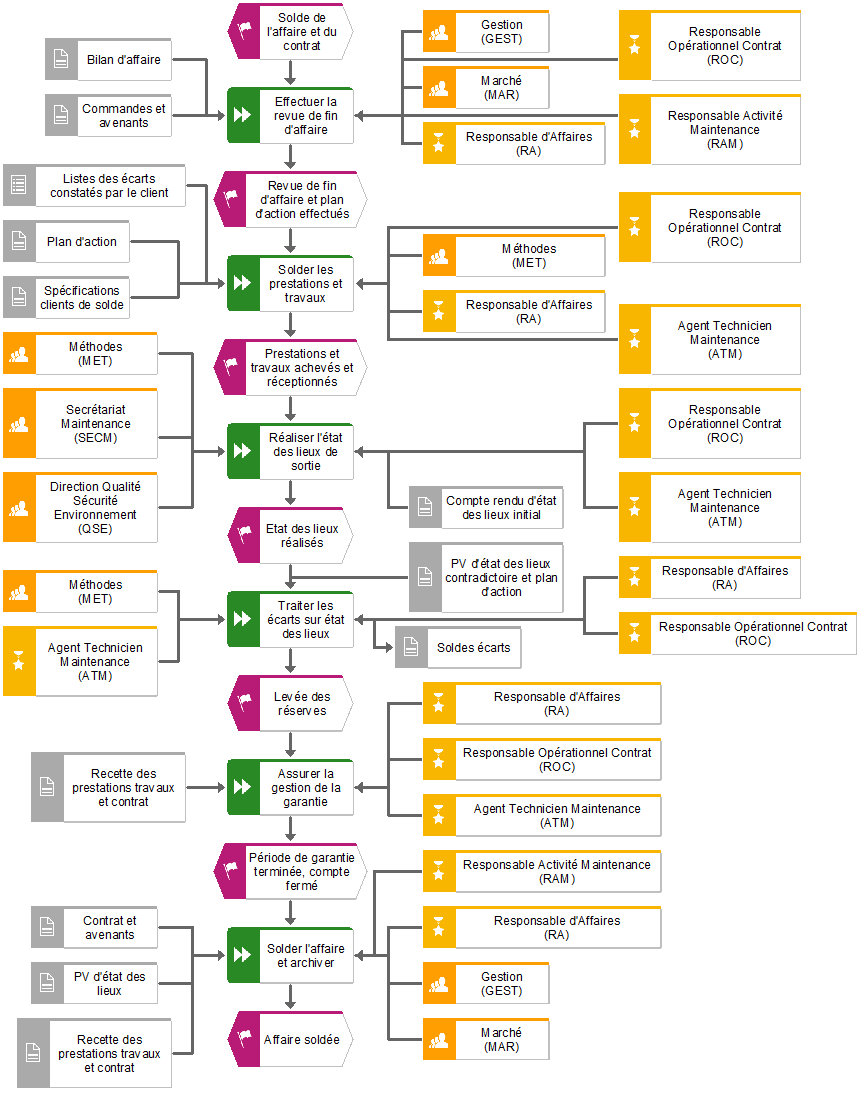
\includegraphics[width=14cm]{figures/aris/soldes_affaire_et_contrat.png}}
    \caption{Processus Soldes Affaire et Contrat}
\end{figure}

\chapter{Matrice ARIS}

\begin{figure}[H]
    \label{fig-matrice}
    \noindent\makebox[\textwidth]{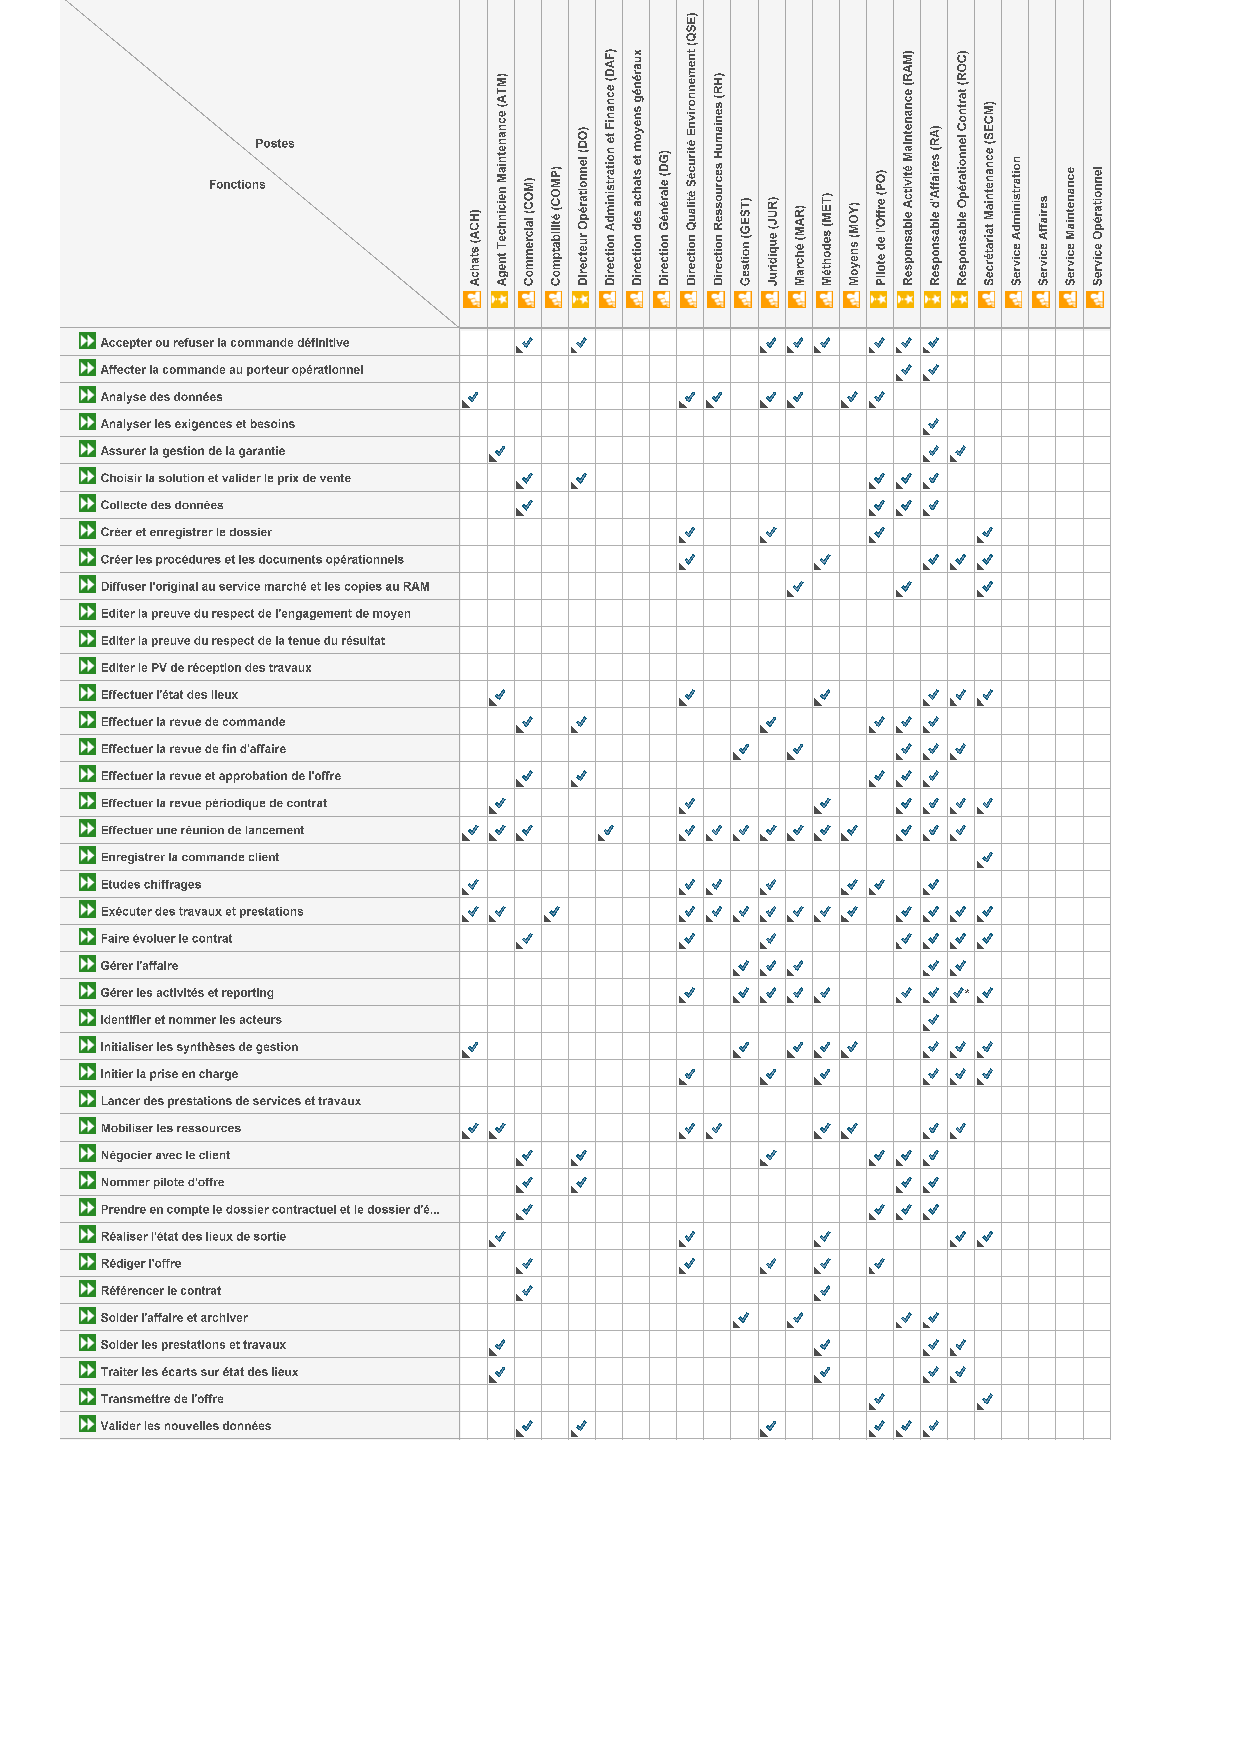
\includegraphics[width=15cm]{pdf_externes/matrice_existant.pdf}}
    \caption{Matrice Fonction - Rôle}
\end{figure}

%%% End document
\end{document}
